
	\documentclass{article}
	\usepackage{amsmath,amssymb}
	\usepackage[inline]{enumitem}
	\usepackage{blindtext}
	\usepackage{booktabs}
	\usepackage{graphicx}
	\usepackage{xcolor}
	\usepackage[vmargin = 1.5in, top = 1in, bottom = 1.2in, letterpaper]{geometry}
	\usepackage{listings}
	\usepackage{courier}
	\usepackage{multicol}
	\usepackage{multirow}
	\usepackage{bm}
	\usepackage{subcaption}
	\usepackage{tabularx}
	\lstset{
	basicstyle = \small\tt,
	keywordstyle = \tt\color{blue},
	commentstyle = \it\color[cmyk]{1,0,1,0},
	stringstyle = \tt\color[RGB]{128,0,0},
	%frame = single,
	backgroundcolor = \color[RGB]{245,245,244},
	breaklines,
	extendedchars = false,
	xleftmargin = 2em,
	xrightmargin = 2em,
	aboveskip = 1em,
	tabsize = 4,
	showspaces = false
	}
	\begin{document}
	
	% \newfontfamily\courier{Courier New}

	
	\title{STAT 557 Homework 4}
	\author{Yifan Zhu}
	\maketitle
	
	\begin{enumerate}[leftmargin = 0 em, label = \arabic*., font = \bfseries]
	\item 
	\begin{enumerate}
		\item
		The fitted result is shown in the table below. From the table we can see only sex and age are significant in this model and thus appear to be associated with the incidence of bile duct hyperplasia.

		\begin{center}
		\begin{tabular}{lllll}
		 \toprule
         		    &Estimate &Std.Error &$z$ value& Pr($>|z|$)\\
         		    \midrule   
         Intercept  & 2.641695&   2.170701&   1.217&  0.22361\\
         tier2      & 0.223906&   0.445897&   0.502&  0.61556\\
         tier3      & 0.442747&   0.434731&   1.018&  0.30847\\
         tier4      & 0.313559&   0.435332&   0.720&  0.47136\\
         tier5      & 0.561481&   0.450625&   1.246&  0.21276\\
         sex        &-1.220903&   0.496367&  -2.460&  \textbf{0.01391}\\
         weight     &-0.007937&   0.015552&  -0.510&  0.60981\\
         age        &-0.029098&   0.009029&  -3.223&  \textbf{0.00127}\\
         pbb        & 0.029886&   0.040542&   0.737&  0.46104\\ 
         \bottomrule
		\end{tabular}
		\end{center}

		\item 
		The sex is code as 1 for female and 0 for male. So $\beta_5 = -1.22$ means with all other conditions the same, the log odd for female to get a bile duct hyperplasia is 1.22 lower than that of male.

		The 95\% interval for $\beta_5$ is
		\[(-2.1937823, -0.2480237)\]
		so the 95\% for $\exp(\beta_5)$ is
		\[(0.1114942, 0.7803415)\]
		\item
		$\beta_8$ has an estimated value 0.029886, which means with all other conditions the same, by increasing 1 unit of pbb, the log odd of getting bile duct hyperplasia would increase by 0.029886. 

		The 95\% interval for $\beta_5$ is
		\[(-0.04957632,  0.10934832)\]
		so the 95\% for $\exp(\beta_5)$ is
		\[(0.9516325, 1.1155509)\]

\newpage
		\item The Pearson and Deviance residual plots with smooth curves are shown below.
		\begin{figure}[!htb]
		\centering
			\begin{subfigure}[b]{0.3\textwidth}
			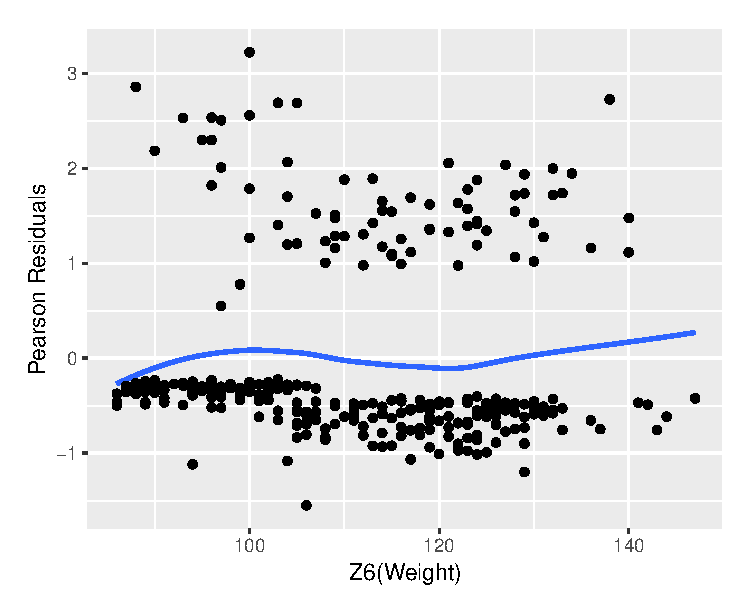
\includegraphics[width = \textwidth]{pz6.eps}
			\end{subfigure}%
			\begin{subfigure}[b]{0.3\textwidth}
			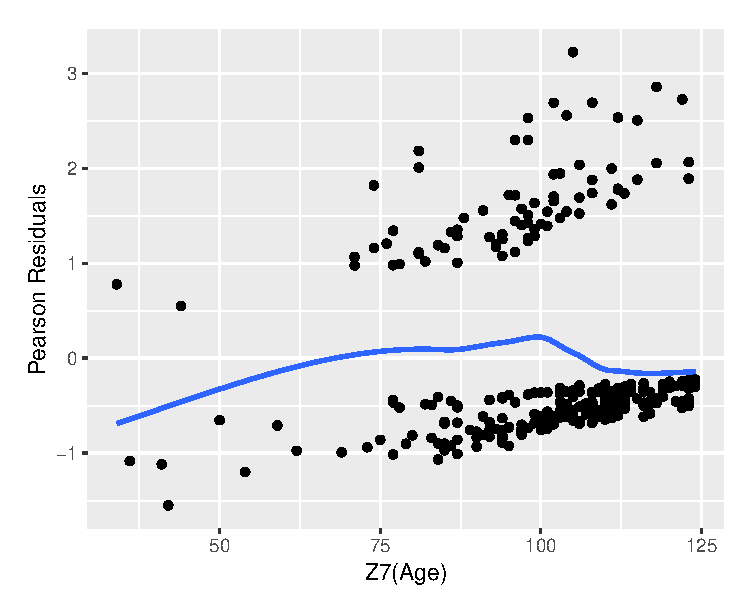
\includegraphics[width = \textwidth]{pz7.eps}
			\end{subfigure}%
			\begin{subfigure}[b]{0.3\textwidth}
			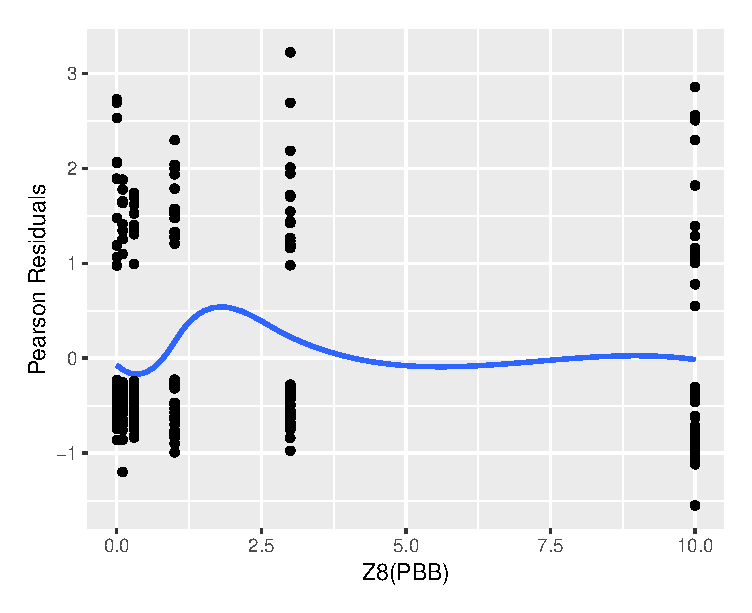
\includegraphics[width = \textwidth]{pz8.eps}
			\end{subfigure}%

			\begin{subfigure}[b]{0.3\textwidth}
			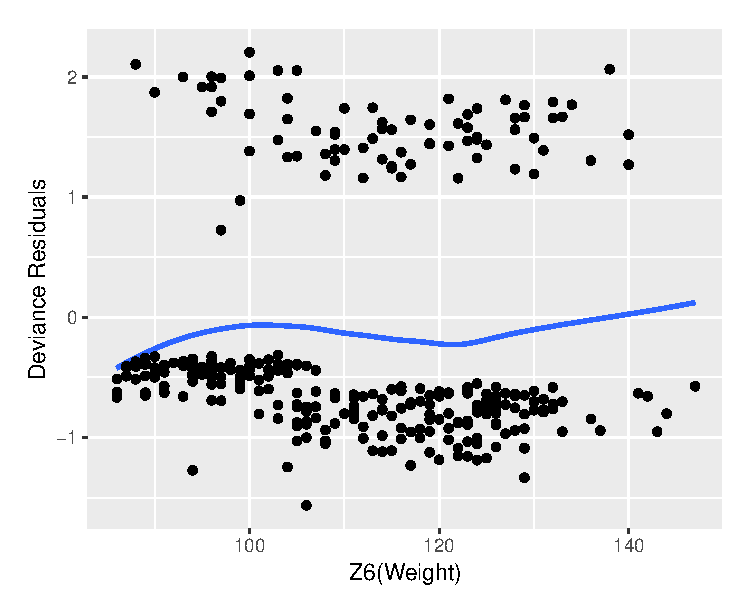
\includegraphics[width = \textwidth]{dz6.eps}
			\end{subfigure}%
			\begin{subfigure}[b]{0.3\textwidth}
			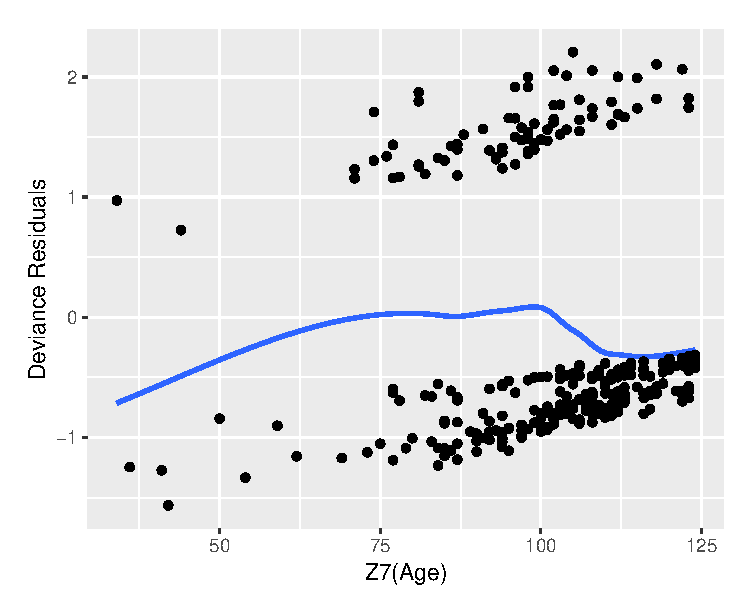
\includegraphics[width = \textwidth]{dz7.eps}
			\end{subfigure}%
			\begin{subfigure}[b]{0.3\textwidth}
			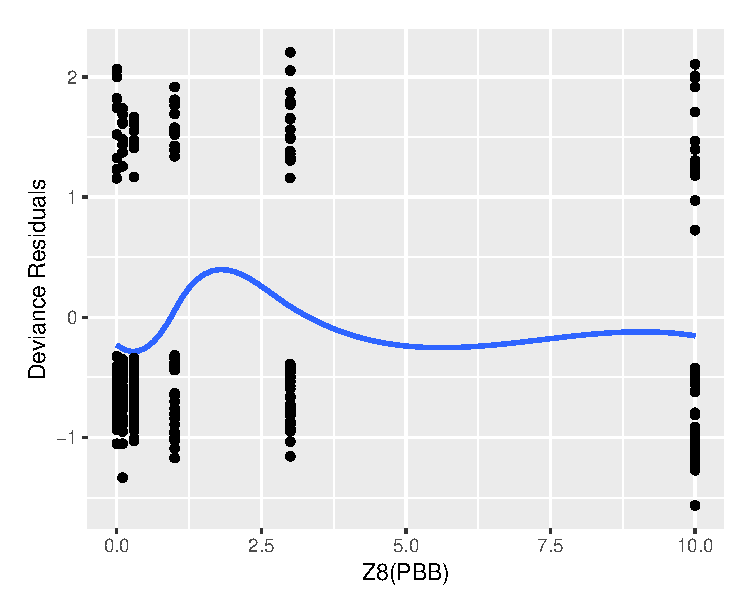
\includegraphics[width = \textwidth]{dz8.eps}
			\end{subfigure}
		\end{figure}

		The smooth curves are not flat and suggest the model does not fit the data well.

		 \item 
		 Using stepwise selection and start with the model with $Z_5 Z_6, Z_5 Z_7, Z_5 Z_8, Z_6 Z_7, Z_6 Z_8, Z_7 Z_8$. The \verb|step| function in are end up with the model with $Z_5 Z_7, Z_5 Z_8, Z_6 Z_7, Z_6 Z_8, Z_7 Z_8$ added to the model in (a). PBB in this model is significant and has positive estimate, thus it suggests increased PBB increases the risk of bile duct hyperplasia. 

		\begin{center}
		\begin{tabular}{lllll}
		 \toprule
         		    &Estimate &Std.Error &$z$ value& Pr($>|z|$)\\
         		    \midrule   
        Intercept   &38.238171  &15.385454  & 2.485  &0.01294\\ 
        tier2       & 0.339782  & 0.458687  & 0.741  &0.45883\\ 
        tier3       & 0.454982  & 0.449678  & 1.012  &0.31164\\ 
        tier4       & 0.595394  & 0.449606  & 1.324  &0.18542\\ 
        tier5       & 0.753045  & 0.465302  & 1.618  &0.10558\\ 
        sex         &-7.668968  & 3.237539  &-2.369  &0.01785\\ 
        weight      &-0.287320  & 0.126967  &-2.263  &0.02364\\ 
        age         &-0.363190  & 0.146640  &-2.477  &0.01326\\ 
        \textbf{pbb}         &-1.524012  & 0.672345  &-2.267  &\textbf{0.02341}\\ 
        sex:age     & 0.051360  & 0.030589  & 1.679  &0.09315\\ 
        sex:pbb     & 0.434339  & 0.154426  & 2.813  &0.00491\\ 
        weight:age  & 0.002619  & 0.001210  & 2.165  &0.03040\\ 
        weight:pbb  & 0.007860  & 0.005022  & 1.565  &0.11758\\ 
        age:pbb     & 0.005695  & 0.002365  & 2.409  &0.01601\\ 
         \bottomrule
		\end{tabular}
		\end{center}  

\newpage
		\item 
		From the plot of leverage against id and influence (c) against id, we can there are several potential extreme covariate value and outliers, roughly for id around 0, 100 and 300.
		\begin{figure}[!htb]
		    \centering
			\begin{subfigure}[b]{0.5\textwidth}
			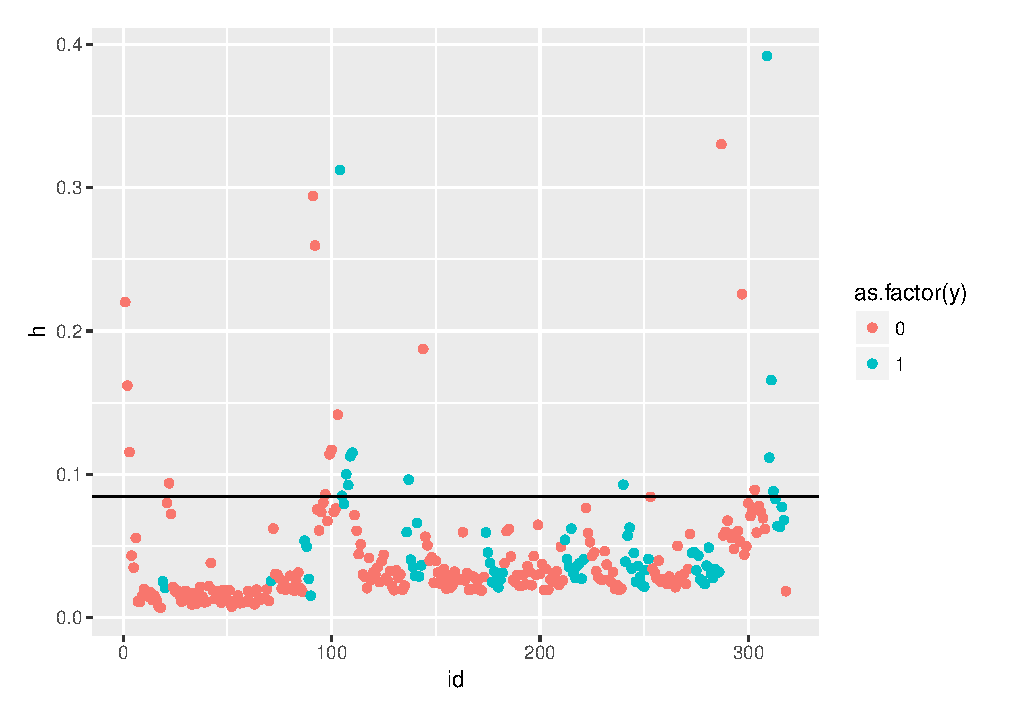
\includegraphics[width = \textwidth]{leverage.eps}
			\end{subfigure}%
			\begin{subfigure}[b]{0.5\textwidth}
			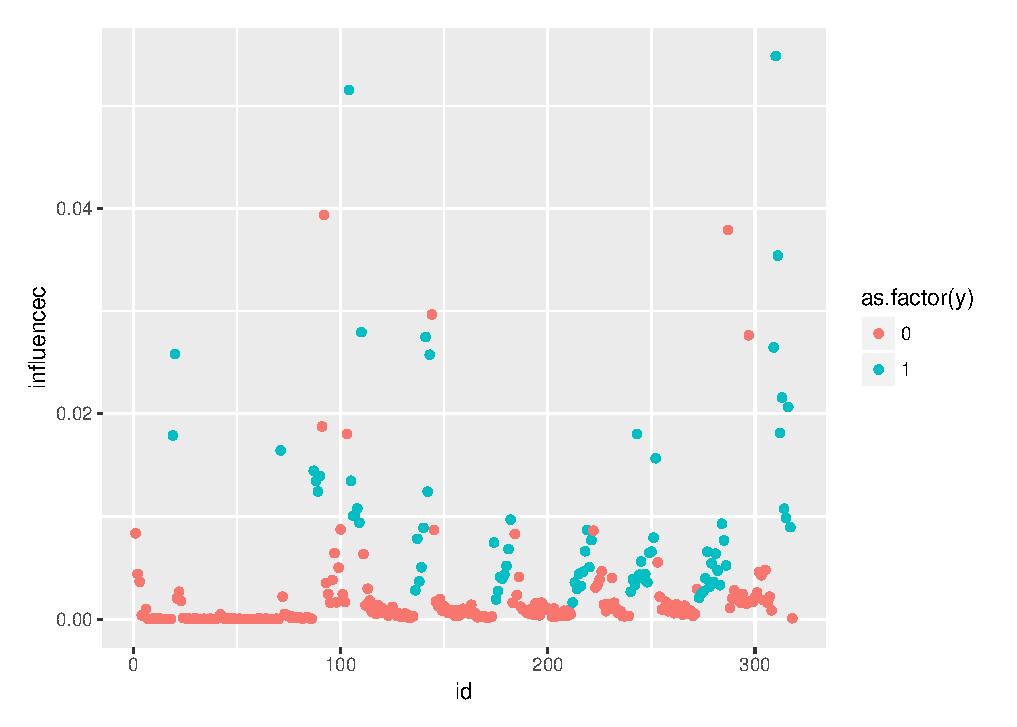
\includegraphics[width = \textwidth]{influence.eps}
			\end{subfigure}
		\end{figure}

		\item 

		\item 


		
	
	

	
	
	\end{enumerate}
\newpage
	\item 
	\begin{enumerate}
		\item
		\begin{enumerate}
		\item The value of log-likelihood ratio $G^2 = 24.3237$. The degrees of freedom is 12 and p-value is 0.0183736. With small p-value, we conclude that the model does not fit the data well.
		
				\item 
				The estimated $\hat{\alpha}_0 = -2.96174, \hat{\alpha}_1 = 0.05521$. 
		
				For $\alpha_0$, it means for people in Denmark at age 16, the log ratio of divorced probability vs married probability is $\alpha_0$ and estimated to be -2.96174.
		
				For $\alpha_1$, it means with 1 year increasing in age, for people in Denmark the log ratio of divorced probability vs married probability would  increase by $\alpha_1$ and estimated to be 0.05521.
		
				\item From the plot we can see the single probability and deviate from the data a lot. And for married probability the model does not fit the data well for small age under 40. The fit of divorced probability is pretty good.
				\begin{figure}[!htb]
					\centering
					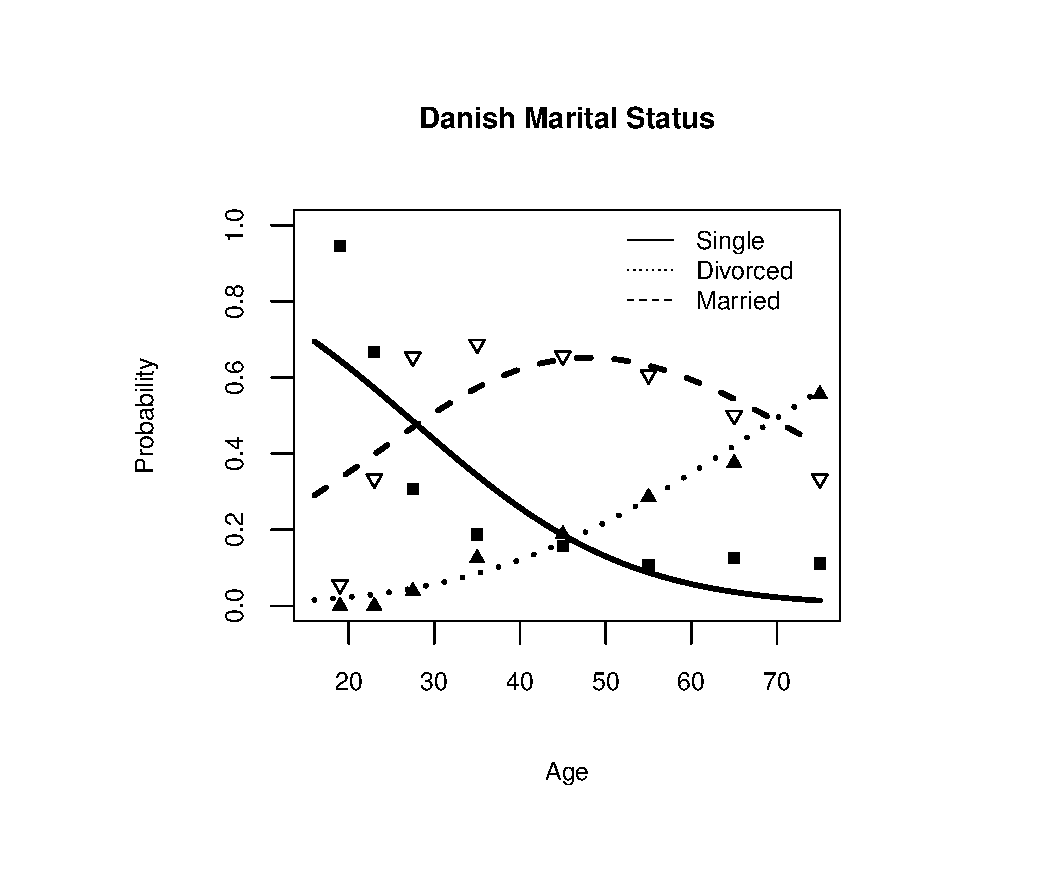
\includegraphics[width = 0.8\textwidth]{2A.eps}
				\end{figure}

		\end{enumerate}
\newpage
		\item 
		\begin{enumerate}
		
		\item The value of log-likelihood ratio $G^2 = 8.6595$. The degrees of freedom is 10 and p-value is 0.564694. With large but not close to 1 p-value, we conclude that the model fit the data somehow well.
		\item From the plot we can see the married probability is fitted a lot better than the previous model. The single probability is fitted well for small age, which is a lot better than the previous model. The divorced probability is also fitted well for small age, but not very well for large age. 
				\begin{figure}[!htb]
					\centering
					\includegraphics[width = 0.75\textwidth]{2B.eps}
				\end{figure}


		\end{enumerate}
\newpage
		\item 
		\begin{enumerate}
			\item The value of log-likelihood ratio $G^2 = 7.8249$. The degrees of freedom is 12 and p-value is 0.7986598. With large but not close to 1 p-value, we conclude that the model fit the data somehow well.
		\item From the plot we can see the three probability lines are all fitted pretty well. And for large age the divorced probability and single probability are fitted better than model B. Also for age around 30 to 40, the married probability is fitted better then that of model B.
						\begin{figure}[!htb]
					\centering
					\includegraphics[width = 0.8\textwidth]{2C.eps}
				\end{figure}

		\end{enumerate}

\newpage
		\item 
		\begin{enumerate}
			\item The value of log-likelihood ratio $G^2 = 1.7077$. The degrees of freedom is 10 and p-value is 0.9981293. With large and close to 1 p-value, we conclude that the model fit the data pretty well.
		\item From the plot we can see the three probability lines are all fitted really well and a lot better than the previous 3 models. 
						\begin{figure}[!htb]
					\centering
					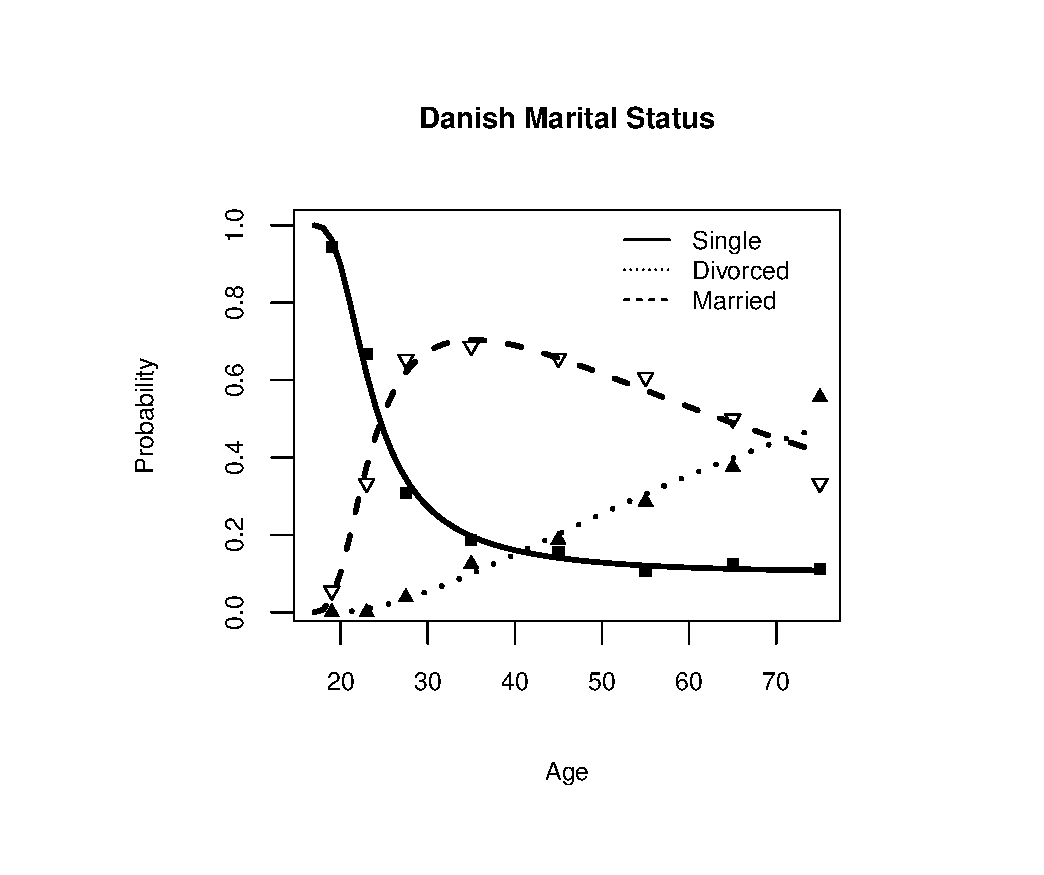
\includegraphics[width = 0.8\textwidth]{2D.eps}
				\end{figure}

		\end{enumerate}
		
		\item The table is shown below. From the table we can see model D has the smallest deviance, AIC and SC. But model C also has small AIC and BIC, which are close to those of model D, and the number of parameters for model C is smaller than that of model D. However the deviance of model D is a lot smaller than that of model C, so I think it is worth to add more parameters. And from the plot we can see model D gives the best fitting of data. What's more, 6 is not to many for number of parameters, hence I think model D is the best.  

		\begin{center}
		\begin{tabular}{lllll}
				 \toprule
				 Model & No. Parameters & Deviance & AIC & SC (BIC)\\
				 \midrule
				 A & 4 &  24.32368 &73.03223 & 73.34999 \\
				 B & 6 &  8.659453 &61.367997& 61.844646\\
				 C & 4 &  7.824851 &56.533395& 56.851161\\
				 D & 6 &  1.707711 &54.416255& 54.892904\\
				 \bottomrule
				\end{tabular}
		\end{center}
        
		

	\end{enumerate}
	
	\end{enumerate}





	
	
	
	\end{document}